\documentclass{standalone}

\usepackage{graphics}
\usepackage[dvipsnames,svgnames]{xcolor}

\usepackage{tikz,pgf,pgfplots,circuitikz}
\pgfplotsset{compat=1.15}
\usetikzlibrary{intersections,arrows.meta,angles,calc,3d,decorations.pathmorphing}

\usepackage{amssymb,amsfonts,amsthm,mathtools}
\usepackage{physics,braket,bm}

\begin{document}  
  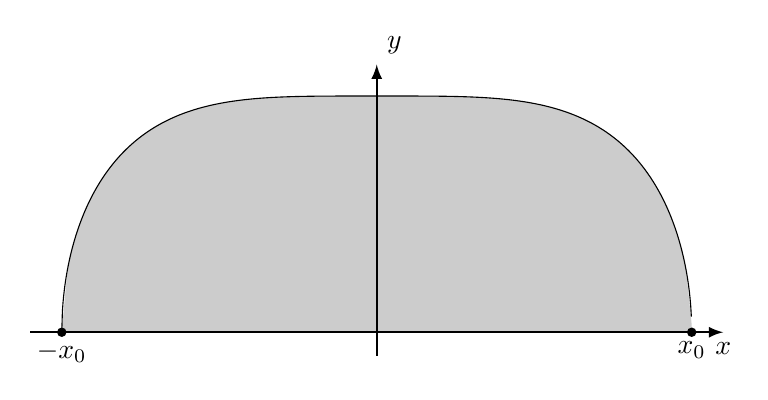
\begin{tikzpicture}
    \fill[opacity=0.2] plot [smooth,samples=100,domain=-4:4] (\x,{sqrt(abs(4*4*4*4-\x*\x*\x*\x))/16*3}) -- (4,0) -- (-4,0);
    \draw[-latex,thick] (-4.4,0)--(4.4,0) node [below]{$x$};
    \draw[-latex,thick] (0,-0.3)--(0,3.4) node [above right] {$y$};
    \draw[name path=int, domain=-4:4,samples=1000] plot (\x,{sqrt(abs(4*4*4*4-\x*\x*\x*\x))/16*3});
    \fill(-4,0)circle(0.06)node[below]{$-x_0$};
    \fill(4,0)circle(0.06)node[below]{$x_0$};
  \end{tikzpicture}
\end{document}
